\documentclass[10pt,a4paper]{article}\usepackage[margin=16mm]{geometry}\usepackage{fontspec,amsmath,graphicx,booktabs}\setmainfont{Latin Modern Roman}\setlength{\parindent}{0pt}\setlength{\parskip}{6pt}\begin{document}
{\Large Five-mode versus general stationary fields: background caps}\par 6 October 2026

Six joint two-window fits. Same pooled inverse-gain calibration, unchanged transmission matrix, uniform final-arc references, cyclic-offset correspondence and measured-total-normalized channel objective. No signal-relative weighting. One background field is shared across both windows; cone geometry, brightness and offset are window-specific.

Both families have a stationary coherent pupil field plus a noninterfering Stokes background. Five-mode uses the earlier two uniform-polarization and three dipole-derived vector modes (five complex coefficients); general uses ten complex transverse pupil modes spanning signal overlaps. Both are evaluated on the same optical quadrature and annular Fresnel/BFP model. Pair sums hold by construction. Different finite bases need not have literally nested background-power representations; comparison here is of the implemented physical families.

Background caps refer to the smaller of the two original, gain-corrected training maxima, so the shared background satisfies the stated cap in both windows. Broad cap retains the previous 95\% of the stricter original minimum total intensity (about 56\% of the smaller maximum). The actual fitted BG percentage is reported below, separately for each window.
\[
J=\sum_{ij}(\varepsilon_{ij}/T_j^{train})^2+
100\sum_j\left[\max\left(0,\frac{\widehat r_j-r_{max}}{1-r_{max}}\right)\right]^6+
10\sum_{ij}[\min(0,\widehat S_{ij})/T_j^{train}]^2.
\]
Here $\widehat S=I^{train}-B-L(d^{fit})$. The radial term has a numerical denominator guard near zero pair intensity; raw corrected intensities are used for diagnostics. Penalties use training data only. Multiple starts and 8192-point refinement are used; convergence is reported, not a global-optimum guarantee.

\begin{tabular}{llrrrrr}\toprule
Model/cap & Window & BG\% & Meas. RMS & Signal RMS & Invalid & Conv.\\\midrule
5 / broad & 30s & 55.5 & 0.0064 & 0.0265 & 21 & yes \\
5 / broad & 10s & 55.3 & 0.0104 & 0.0297 & 14 & yes \\
5 / 10pct & 30s & 10.0 & 0.0249 & 0.0347 & 0 & yes \\
5 / 10pct & 10s & 10.0 & 0.0272 & 0.0352 & 0 & yes \\
5 / 5pct & 30s & 5.0 & 0.0327 & 0.0433 & 0 & yes \\
5 / 5pct & 10s & 5.0 & 0.0347 & 0.0427 & 0 & yes \\
10 / broad & 30s & 52.8 & 0.0049 & 0.0324 & 16 & yes \\
10 / broad & 10s & 52.6 & 0.0097 & 0.0467 & 19 & yes \\
10 / 10pct & 30s & 10.0 & 0.0114 & 0.0139 & 0 & no \\
10 / 10pct & 10s & 10.0 & 0.0144 & 0.0175 & 0 & no \\
10 / 5pct & 30s & 5.0 & 0.0196 & 0.0227 & 0 & yes \\
10 / 5pct & 10s & 5.0 & 0.0231 & 0.0261 & 0 & yes \\
\bottomrule\end{tabular}

RMS values are four-channel residuals divided by measured total or fitted signal total respectively. Signal RMS is diagnostic only. Invalid counts include negative corrected channels or $r>r_{max}$. Signal-space curves show conditional fitted-interference subtraction, not self-consistent field inversion. Red triangles indicate points beyond fixed axes. A low cap may improve subtraction stability while worsening measured-space agreement; neither establishes correct rod angles. No commit or push.
\newpage
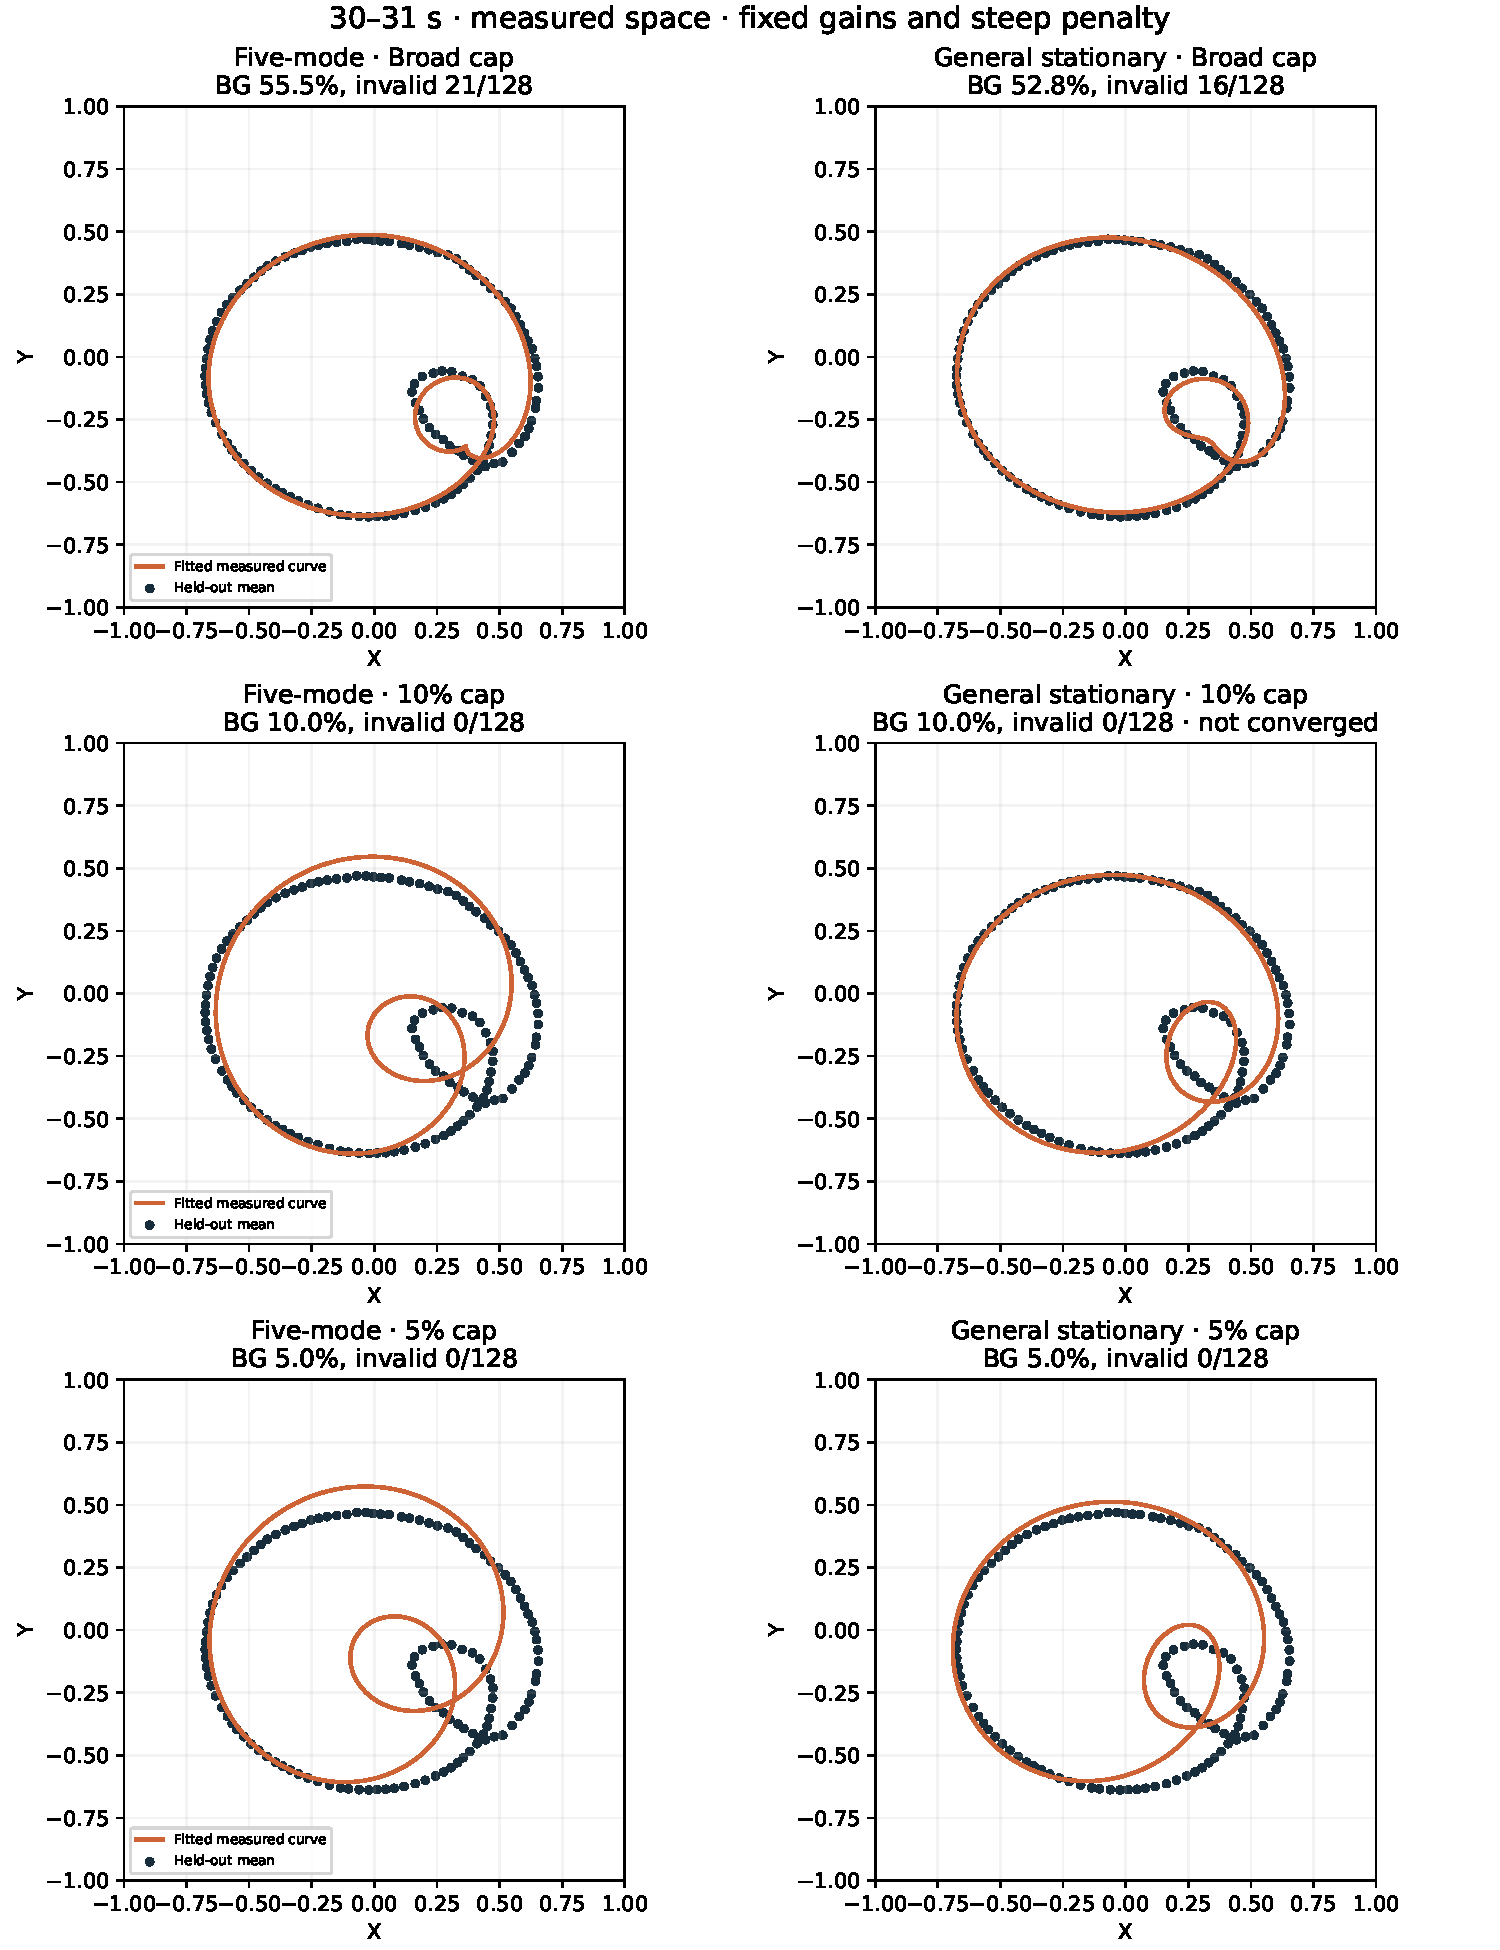
\includegraphics[width=\linewidth,height=.94\textheight,keepaspectratio]{30s_measured.pdf}
\newpage
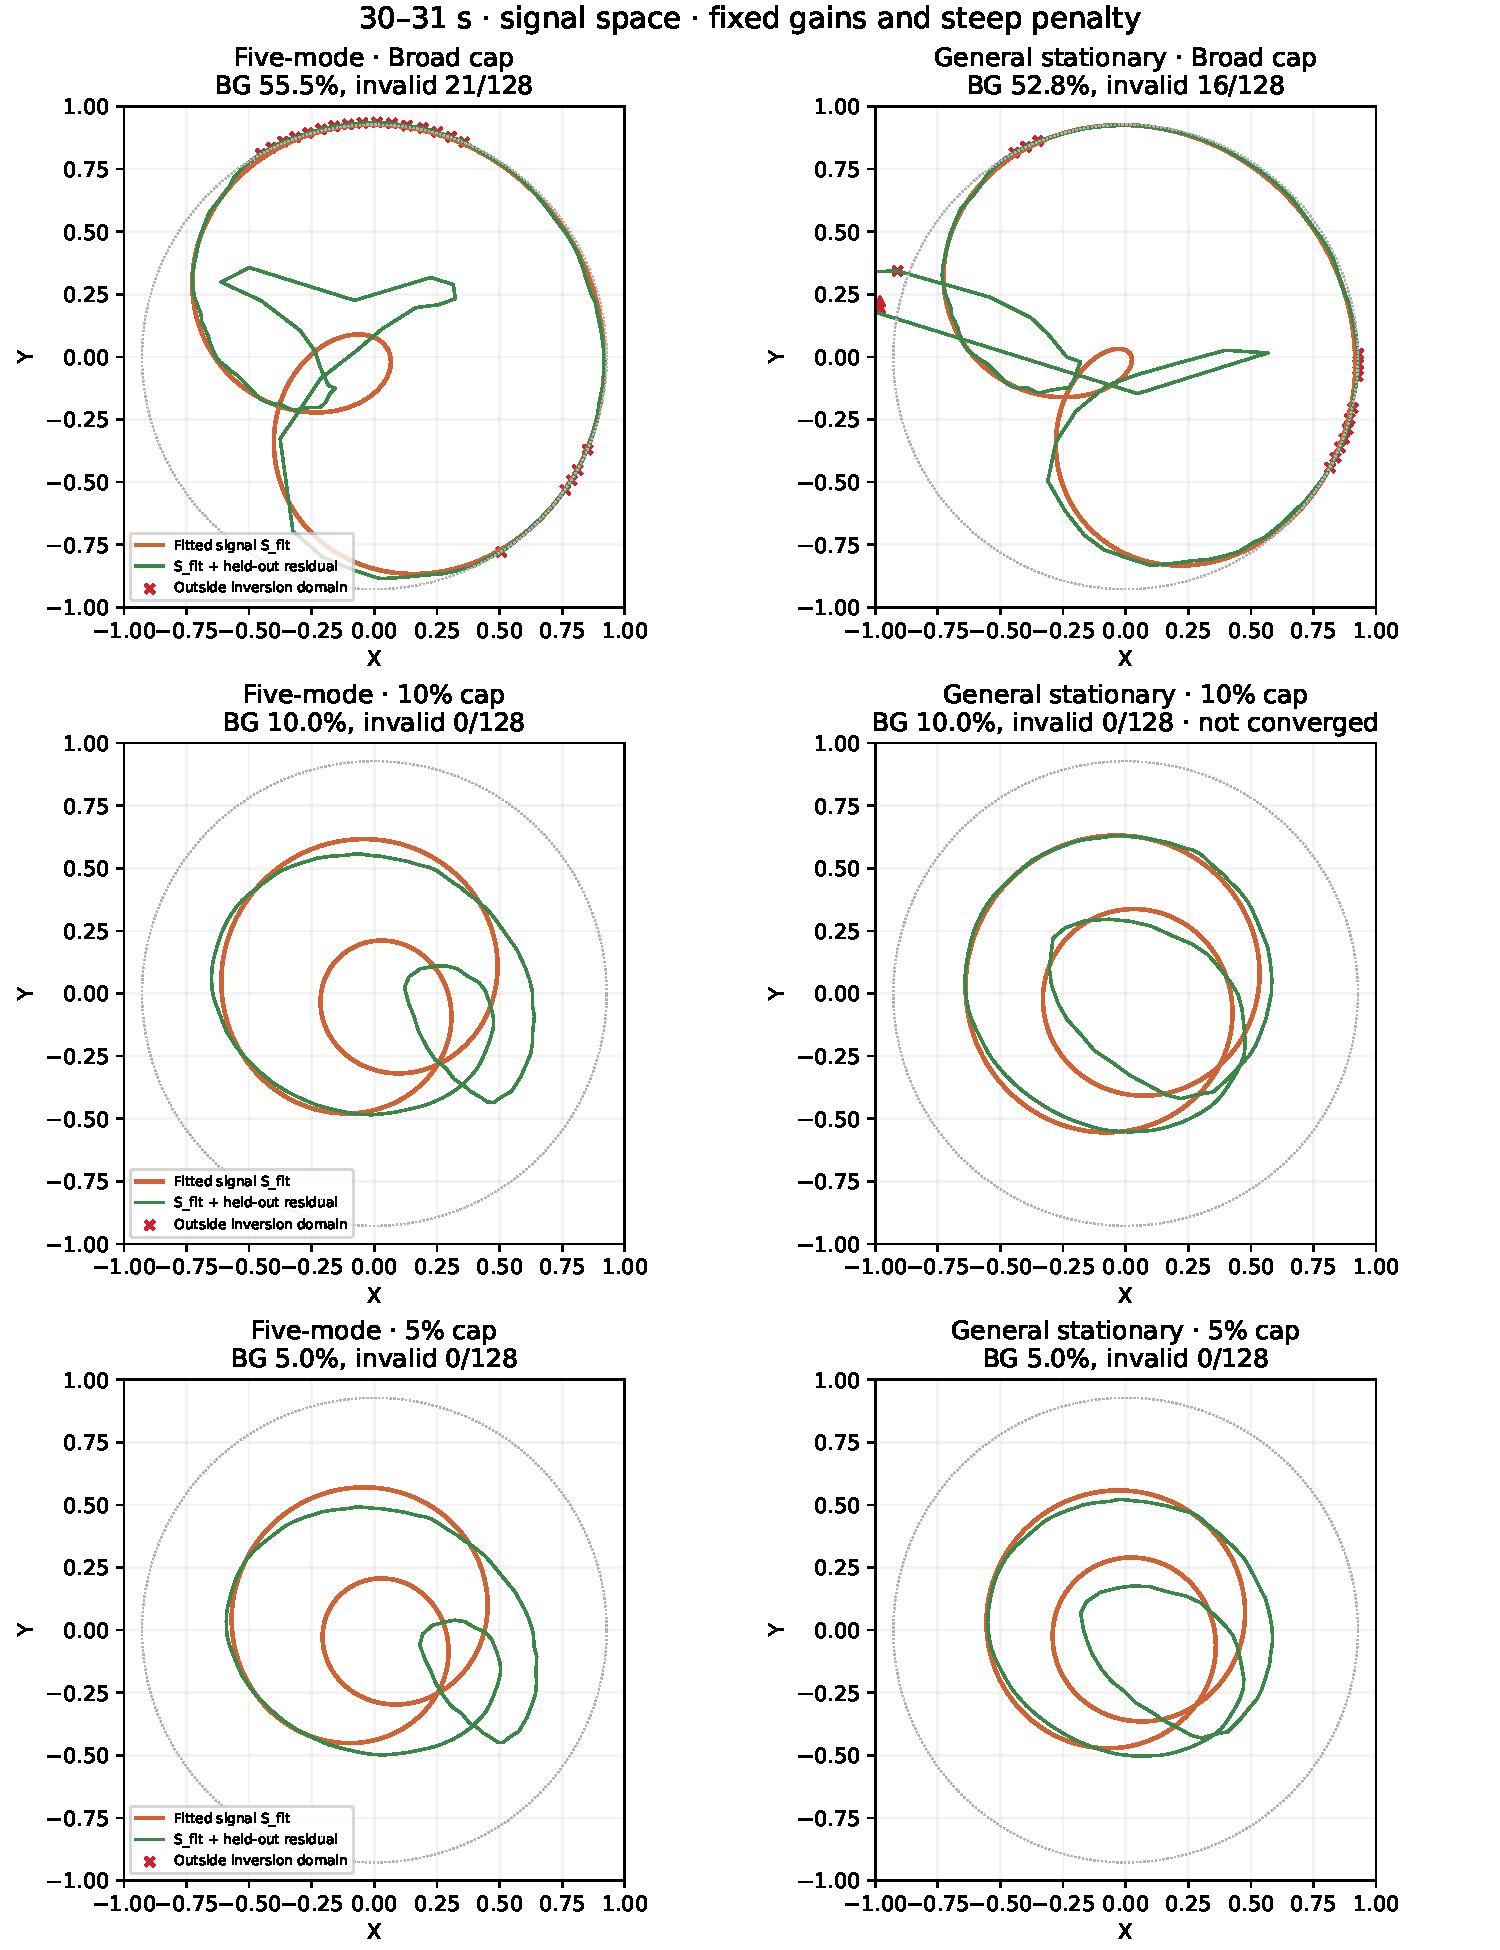
\includegraphics[width=\linewidth,height=.94\textheight,keepaspectratio]{30s_signal.pdf}
\newpage
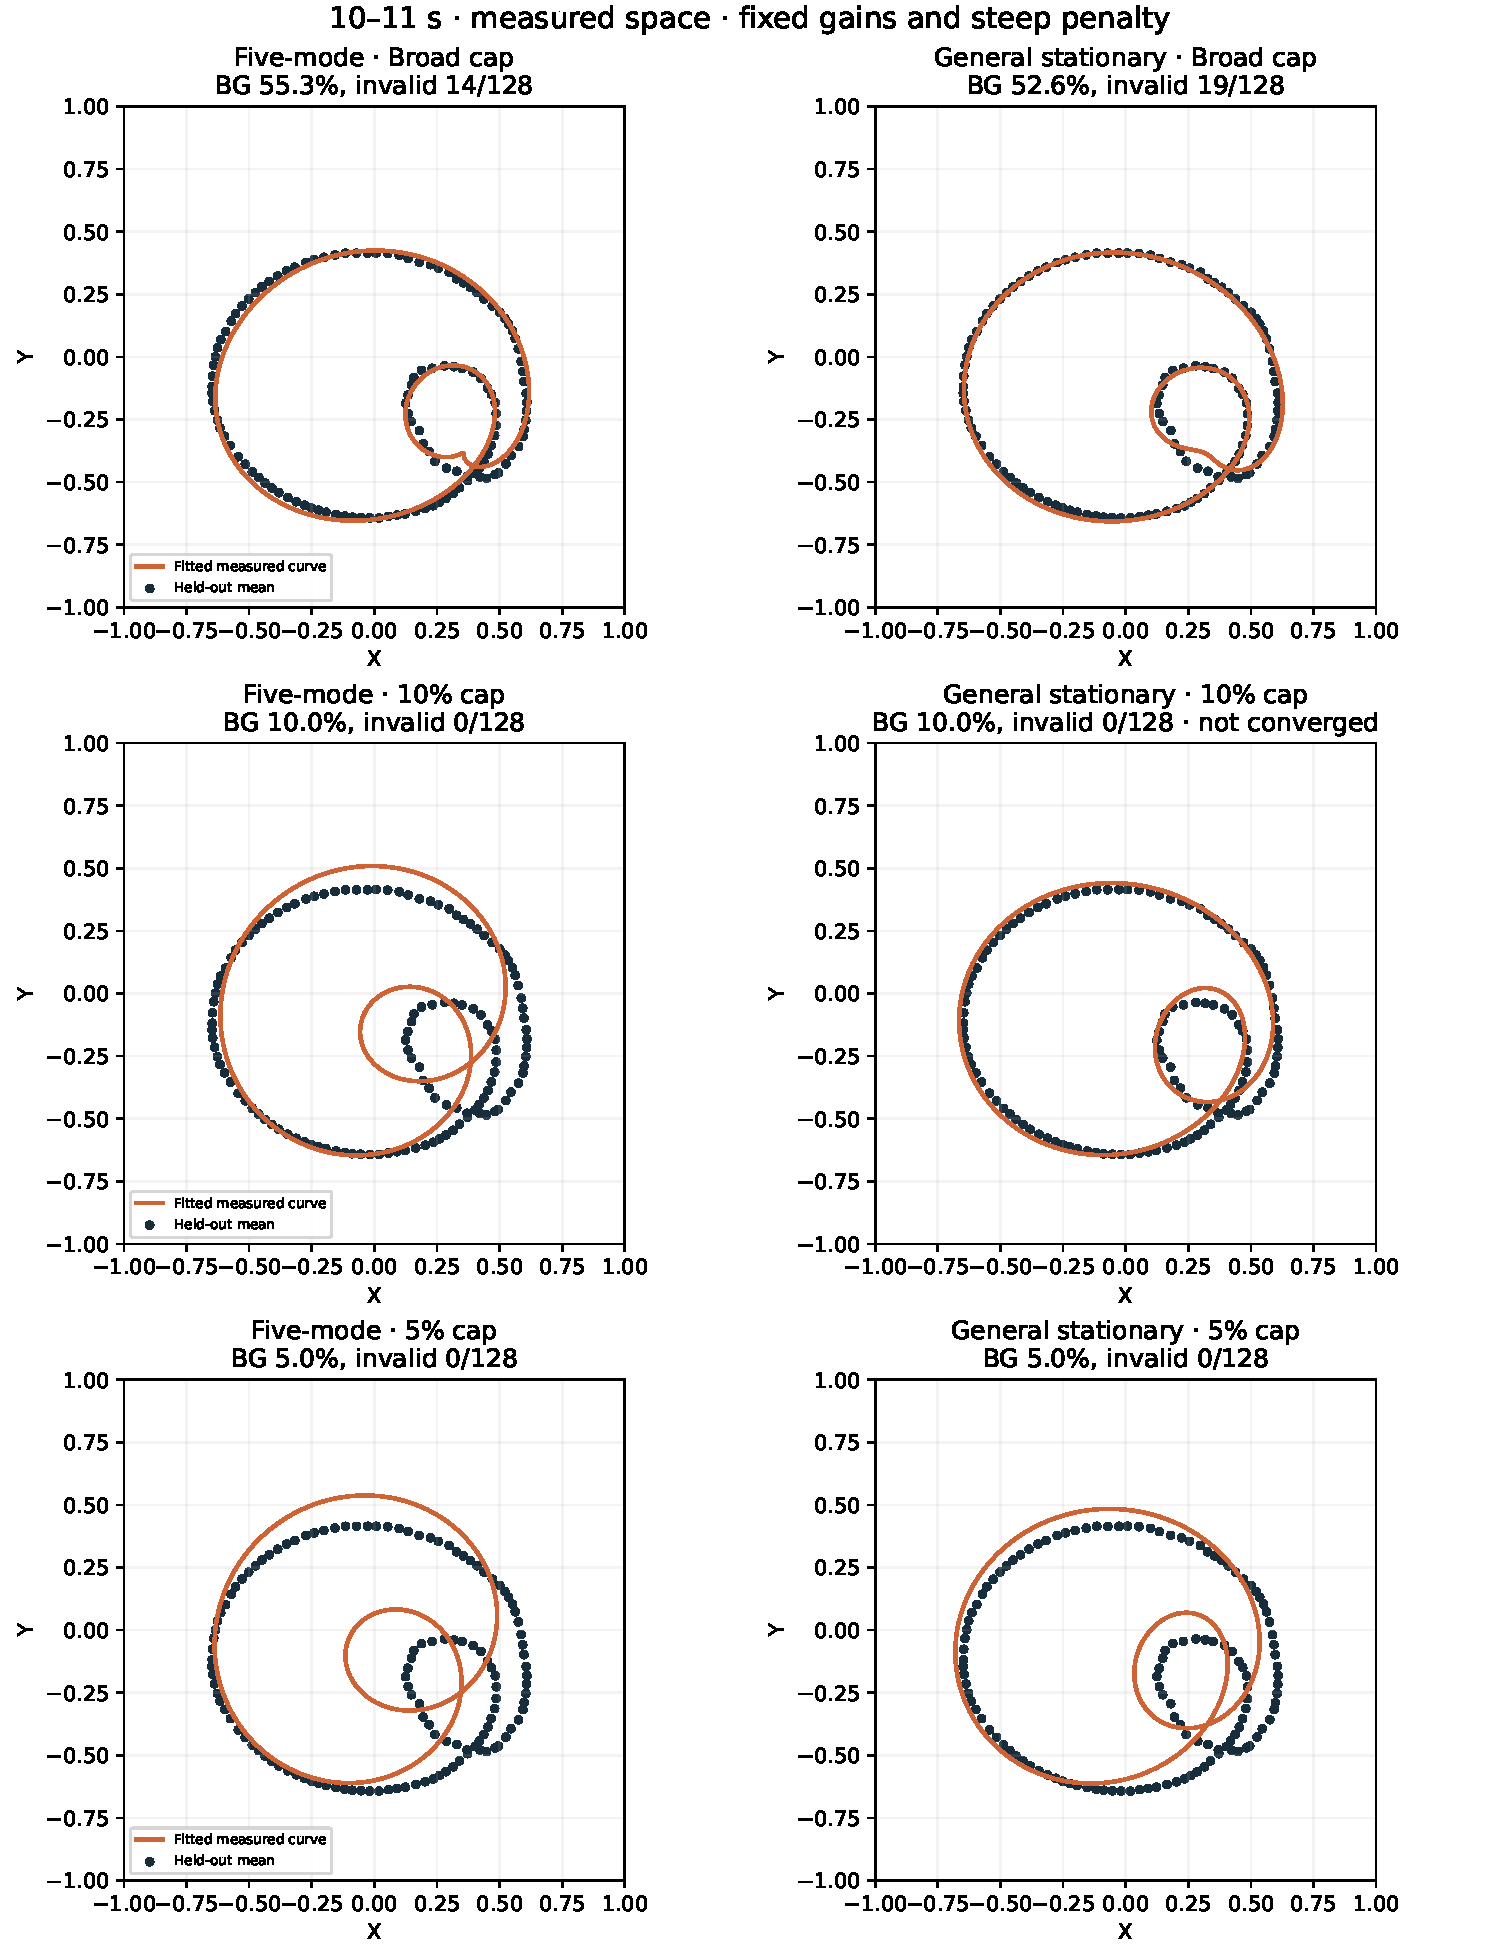
\includegraphics[width=\linewidth,height=.94\textheight,keepaspectratio]{10s_measured.pdf}
\newpage
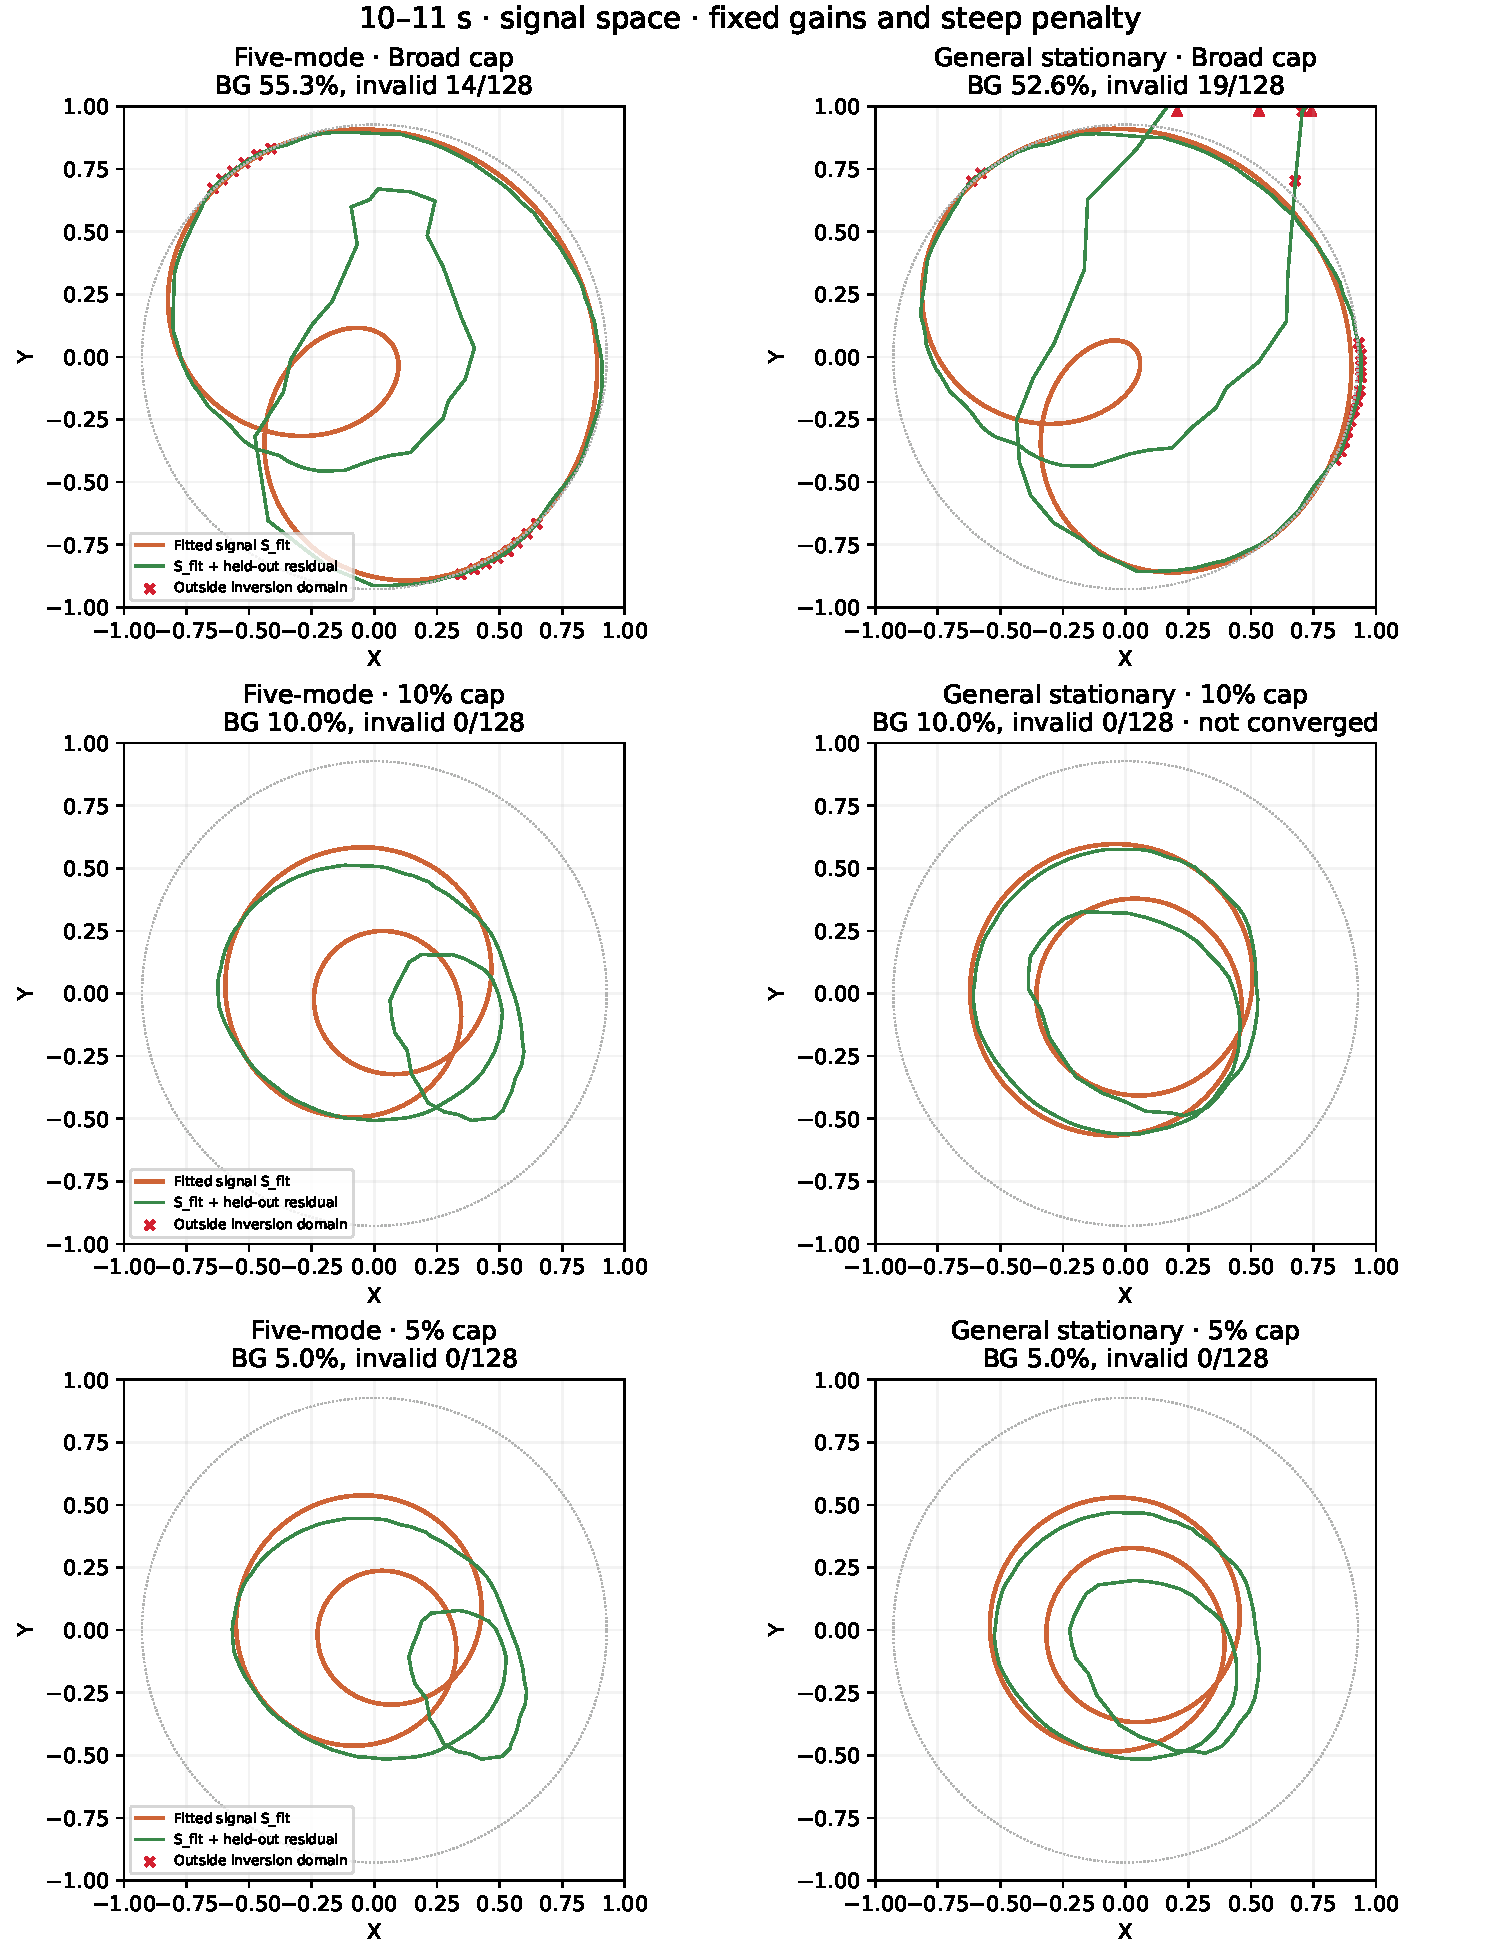
\includegraphics[width=\linewidth,height=.94\textheight,keepaspectratio]{10s_signal.pdf}
\end{document}
